\subsection{Infinite Group}

First, we want to define a representation of an infinite group.
$S^1$ is an easy-to-understand group with a simple structure.
It consists of all rotational symmetries of a circle, like the unit circle in \Cref{fig:infinite.group.unit}.
One \textit{simple} (irreducible) and \textit{faithful} representation is the identification of each rotation with its angle $\theta$.
The (counterclockwise) rotation is represented by the number $e^{\theta i}$.
This representation is one-dimensional and faithful.
We can see that $S^1$ must be abelian since the complex numbers commute under multiplication.
One result of Shur's Lemma introduced in \Cref{sec:reprep.simp} is that all simple representations of abelian groups must be one-dimensional~\cite{hein2013}.


\begin{figure}[!h]
    \centering

    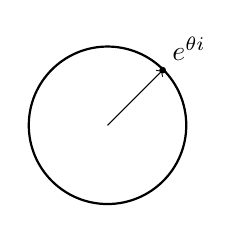
\begin{tikzpicture}
        \draw[thick] (0,0) circle (1);

        \coordinate (z) at (0.7, 0.7);
        \draw[fill] (z) circle (1pt);
        \draw[->] (0,0) -- (z);

        \node[above right] at (z) {$e^{\theta i}$};
    \end{tikzpicture}

    \caption{Unit Circle with a Complex Number}
    \label{fig:infinite.group.unit}
\end{figure}
